\section{Auswertung}
\subsection{Vorselektion}

Um die enorme Datenmenge zu reduzieren wurde eine Vorselektion auf die Daten angewandt.
Diese reduziert die ursprünglich $~ 66 \cdot 10^6$ Events auf $~ 6.6 \cdot 10^6$ Events.
Um diese Reduktion zu erreichen, werden einige Anforderungen an jedes Event gestellt.
Zu Bemerken ist, dass in manchen Größen mehr Einträge zu finden sind, als Events im Tupeln vorhanden sind.
Dies hat den Grund, dass Events mit mehreren Jets oder Leptonen für jeden Jet und jedes Lepton einen separaten Eintrag enthalten.
Dies taucht somit auch nur für Größen auf, die die Eigenschaften der Jets oder Leptonen zeigen.
Zunächst wird gefordert, dass der entsprechende Myon- oder Elektrontrigger ausgelöst wird.
Damit sollen Beiträge von Untergrundleptonen verringert werden.
Niederenergetische Leptonen lassen sich nämlich sehr schlecht vom Untergrund unterscheiden, weswegen eine typische Triggerschwelle für den transversalen Impuls bei $\SI{25}{\giga\electronvolt}$ liegt.
Diese Mindestenergie lässt sich in den Daten direkt erkennen, wie in Abbildung \ref{fig:elec6pt} für das Datentupel \textit{data.06.el} dargestellt.
Da die Tupel nach den jeweiligen Leptonen sortiert sind, wird auch nur der entsprechende Trigger gefordert.
Die Anzahl der rekonstruierten Leptonen sollte mindestens eins enthalten.
Die Pseudorapidität hängt mit dem transversalen Impuls zusammen.
Je geringer der transversale Impuls, desto größer die Pseudorapidität.
Die Pseudorapiditätsverteilung spiegelt allerdings auch einige Detektoreigenschaften wieder.
So werden in dem Gebiet um $\eta \approx \pm 1.5$ weniger Events registriert.
Dies hat den Grund, dass dort Leitungen oder ähnliche nicht detektierenden Elemente verbaut sind.
Die geometrische Akzeptanz des Detektors beträgt also nicht $\SI{100}{\percent}$.
Das Maximum der Pseudorapidität liegt bei $\eta \approx \pm 3$.
Der Azimuthalwinkel $\Phi$ zeigt keine Anforderungen.

\begin{figure}
  \centering
  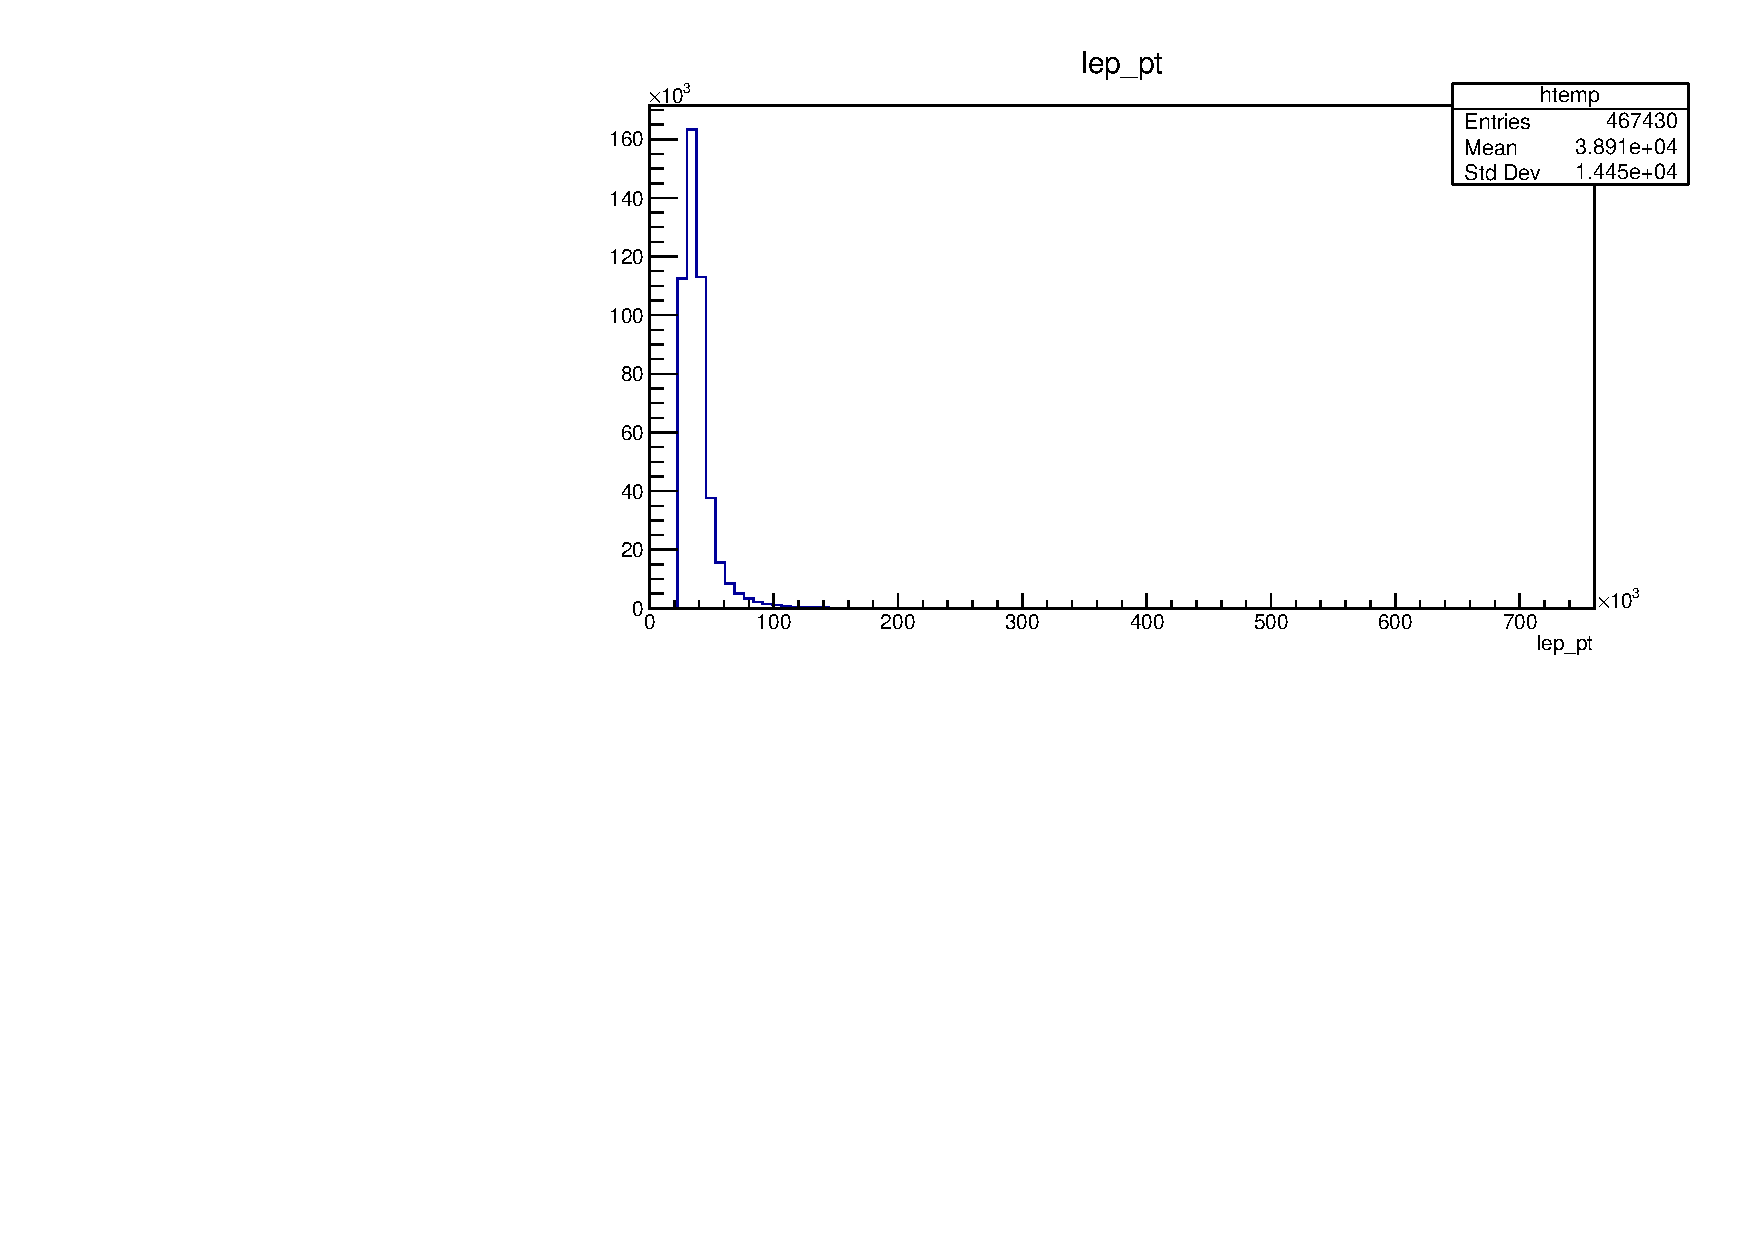
\includegraphics[width=0.8\textwidth]{content/graphics/question2_1/data_electron_6_pt.pdf}
  \caption{Histogramm des transversalen Impulses des Elektrons des Datentupels \textit{data.06.el}.}
  \label{fig:elec6pt}
\end{figure}

\subsection{Erweiterte Eventselektion}

Selektiert wird auf den \texttt{lepton+jets} Kanal. Das bedeutet, es wird genau 
ein geladenes Lepton aus dem leptonischen Zerfall eines $W$-Bosons gefordert. 
Dieses Lepton, soll einen Transversalimpuls von mindestens $\texttt{lep$\_$pt} \textgreater 
\SI{50}{\giga\electronvolt}$ besitzen. Leptonen mit geringerem Transversalimpuls 
werden verworfen. In dem leptonischen Verfall, wird zudem ein 
Neutrino produziert. Daher wird eine fehlende Transversalenergie von 
$\texttt{met$\_$et} \textgreater \SI{40}{\giga\electronvolt}$ gefordert. \par 
Da beide Top-Quarks in ein $W$-Boson mit einem Bottom-Quark zerfallen, entstehen
dadurch bereits zwei Quarks. Aus dem hadronischen Zerfall des zweiten $W$-Bosons 
entstehen zwei weitere Quarks, weswegen in der Selektion Events mit 
$\texttt{jet$\_$n} \textless 4$ verworfen werden. Von diesen Jets, werden 
mindestens zwei Jets verlangt, die b-tagged sein müssen. Das wird dadurch erreicht,
indem ein \texttt{MV1} Wert größer als $0.7892$ gefordert wird. Weiterhin soll 
jeder Jet mindestens einen Transversalimpuls von $\texttt{jet$\_$pt} 
\textgreater \SI{100}{\giga\electronvolt}$ besitzen. \par 
Die Pseudorapidität ist sowohl eine Detektorkomponente als auch eine 
Teilcheneigenschaft, denn Teilchenmasse und -energie beeinflussen den 
Abstrahlungswinkel. Der ATLAS Detektor kann innerhalb eines Akzeptanzbereichs 
von $|{\eta}| \textless 2.4$ messen. Alles was diesen Bereich übersteigt, 
kann nicht von den Detektorkomponenten erfasst werden. Deswegen wird auf 
diese Eigenschaft ebenfalls selektiert. Schnitte auf Teilcheneigenschaften 
wie Transversalimpuls sind notwendig um Untergründe zu reduzieren. Da in diesem 
Versuch ein Teilchen mit hoher invarianter Masse untersucht wird, ist es 
sinnvoll hohe Grenzen auf den Transversalimpuls zu setzen. \par 

Die erwarteten Untergründe für diesen Zerfallskanal sind bereits in 
Kapitel \ref{sec:strategie} gelistet. \par

Zur Berechnung des Koeffizienten $\epsilon * A$, welches für Effizienz mal die 
Detektorakzeptanz steht, wird das Verhälnis der Anzahl der Events, die einen 
Cut überstehen, 
mit der Gesamtanzahl der Events nach der kompletten Selektion gebildet. Dadurch 
ergeben sich für die Samples die in Tabelle \ref{tab:Effizienzen} abgebildeten 
Effizienzen.

\begin{table}
    \centering
    \caption{Berechte Effizienzen für die einzelnen Cuts der Eventselektion}
    \label{tab:Effizienzen}
    \resizebox{\textwidth}{!}{\begin{tabular}{c|cccccc}
    \toprule 
    Sample & $\texttt{lep$\_$n} != 1$ & $\texttt{lep$\_$pt} \textgreater 
\SI{50}{\giga\electronvolt}$ & $\texttt{jet$\_$pt} \textgreater 
\SI{100}{\giga\electronvolt}$ & $\texttt{met$\_$et} \textgreater 
\SI{50}{\giga\electronvolt}$ & $\texttt{btagged} \textgreater 2$ & 
$\texttt{jet$\_$eta} \textless |2.4|$ \\
    \midrule 
    \texttt{ttbar.el}      & 0.9316 & 0.5071  & 0.1406  & 0.0428  & 0.0605  & 0.0400 \\
    \texttt{ttbar.mu}      & 0.9200 & 0.4821  & 0.1340  & 0.0409  & 0.0579  & 0.0382 \\
    \texttt{singletop.el}  & 0.9806 & 0.4323  & 0.0311  & 0.0071  & 0.0103  & 0.0064 \\
    \texttt{singletop.mu}  & 0.9788 & 0.4104  & 0.0288  & 0.0068  & 0.0097  & 0.0062 \\
    \texttt{diboson.el}    & 0.9044 & 0.3813  & 0.0048  & 7.97e-05  & 0.0001  & 7.9691e-05 \\
    \texttt{diboson.mu}    & 0.8731 & 0.3510  & 0.0038  & 7.38902e-05  & 9.99691e-05  & 6.51973e-05 \\
    \texttt{wjets.el}      & 0.9999 & 0.1709  & 0.0017  & 1.39121e-05  & 1.99407e-05  & 1.28301e-05 \\
    \texttt{wjets.mu}      & 0.9999 & 0.1589  & 0.0016  & 1.56505e-05 & 2.33554e-05 & 1.49282e-05 \\
    \texttt{zjets.el}      & 0.7167 & 0.1814  & 0.0032  & 4.8692e-05 & 0.000135906 & 4.59184e-05 \\
    \texttt{zjets.mu}      & 0.5015 & 0.1256  & 0.0014  & 3.18146e-05 & 7.37231e-05 & 3.00259e-05 \\
    \texttt{zprime400.el}  & 0.9308 & 0.4464  & 0.0470  & 0.0124  & 0.0192  & 0.0119 \\
    \texttt{zprime400.mu}  & 0.9201 & 0.4215  & 0.0539  & 0.0137  & 0.0203  & 0.0131 \\
    \texttt{zprime500.el}  & 0.9324 & 0.5616  & 0.1499  & 0.0417  & 0.0625  & 0.0399 \\
    \texttt{zprime500.mu}  & 0.9224 & 0.5353  & 0.1357  & 0.0389  & 0.0581  & 0.0378 \\
    \texttt{zprime750.el}  & 0.9237 & 0.6705  & 0.3503  & 0.1216  & 0.1573  & 0.1155 \\
    \texttt{zprime750.mu}  & 0.9133 & 0.6451  & 0.3332  & 0.1220  & 0.1526  & 0.1173 \\
    \texttt{zprime1000.el} & 0.9339 & 0.7342  & 0.4399  & 0.1789  & 0.2087  & 0.1728 \\
    \texttt{zprime1000.mu} & 0.9182 & 0.7055  & 0.4330  & 0.1681  & 0.2021  & 0.1596 \\
    \texttt{zprime1250.el} & 0.9355 & 0.7475  & 0.4665  & 0.1898  & 0.2157 & 0.1820 \\
    \texttt{zprime1250.mu} & 0.9246 & 0.7319  & 0.4702  & 0.1931  & 0.2217  & 0.1853 \\
    \texttt{zprime1500.el} & 0.9401 & 0.7711  & 0.4905  & 0.1905  & 0.2121  & 0.1819 \\
    \texttt{zprime1500.mu} & 0.9287 & 0.7483  & 0.4902  & 0.1893  & 0.2125  & 0.1805 \\
    \texttt{zprime1750.el} & 0.9473 & 0.7758  & 0.5036  & 0.1932  & 0.2146  & 0.1840 \\
    \texttt{zprime1750.mu} & 0.9383 & 0.7571  & 0.4914  & 0.1898  & 0.2091  & 0.1819 \\
    \texttt{zprime2000.el} & 0.9451 & 0.7629  & 0.4873  & 0.1747  & 0.1913  & 0.1683 \\
    \texttt{zprime2000.mu} & 0.9406 & 0.7611  & 0.5066  & 0.1799  & 0.1968  & 0.1717 \\
    \texttt{zprime2250.el} & 0.9450 & 0.7451  & 0.4839  & 0.1688  & 0.1846  & 0.1588 \\
    \texttt{zprime2250.mu} & 0.9448 & 0.7639  & 0.5085  & 0.1824  & 0.2012  & 0.1738 \\
    \texttt{zprime2500.el} & 0.9480 & 0.7509  & 0.4809  & 0.1598  & 0.1759  & 0.1523 \\
    \texttt{zprime2500.mu} & 0.9433 & 0.7595  & 0.5078  & 0.1765  & 0.1933  & 0.1669 \\
    \texttt{zprime3000.el} & 0.9437 & 0.7151  & 0.4253  & 0.1458  & 0.1648  & 0.1368 \\
    \texttt{zprime3000.mu} & 0.9398 & 0.7314  & 0.4631  & 0.1607  & 0.1781  & 0.1516 \\
    \bottomrule 
    \end{tabular}}
\end{table}

Nach der Eventselektion ist Top-Quark Paarproduktion der größte Untergrund, da die Signatur dieses 
Untergrundes der selektierten Signatur ähnelt.

\subsection{Fundamentale Verteilungen}

Die größe Untergrundquelle sind nach der vollständigen Selektion die $t\bar{t}$-Prozesse.
Um ihre Eigenschaften besser verstehen zu können, wurden einige Größen hier aufgetragen.
Diese werden dann mit den Erwartungen für $t\bar{t}$-Prozesse verglichen.
Dabei handelt es sich um Monte-Carlo Simulationen des $t\bar{t}$-Prozesses mit Myonen.
Einige dieser Größen sind in Abbildung \ref{fig:Distributions} dargestellt.
Der Rest ist im Anhang in Kapitel \ref{sec:reste} in Abbildung \ref{fig:Distributions2} - \ref{fig:Distributions4} zu finden.
Sie stimmen mit den Erwartungen an den $t\bar{t}$-Prozess gut überein.
So ist zum Beispiel in Abbildung \ref{fig:btagged} die Anzahl an btagged Jets zu sehen.
Btagged Jets sind Jets die mit einer gewissen Wahrscheinlichkeit ($MV1 > 0.7892$) ihren Ursprung in einem b-Quark nahmen.
Da in einem $t\bar{t}$-Prozess, wie in Abbildung \ref{fig:gluonfusion} zu sehen, zwei b-Jets erzeugt werden, ist die Verteilung in der Hinsicht wie zu erwarten.
Der restliche transversale Impuls wird dann gleichermaßen auf das Myon und das Neutrino aufgeteilt.
Diese beiden Verteilungen in Abbildung \ref{fig:lep_pt} und \ref{fig:met_et} weisen einen ähnlichen Peak und Verlauf auf.
Allerdings ist die Verteilung durch die fehlende Auflösung für die Neutrinos etwas ausgeschmierter, bzw. flacher.

\begin{figure}
  \begin{subfigure}{0.5\textwidth}
    \centering
    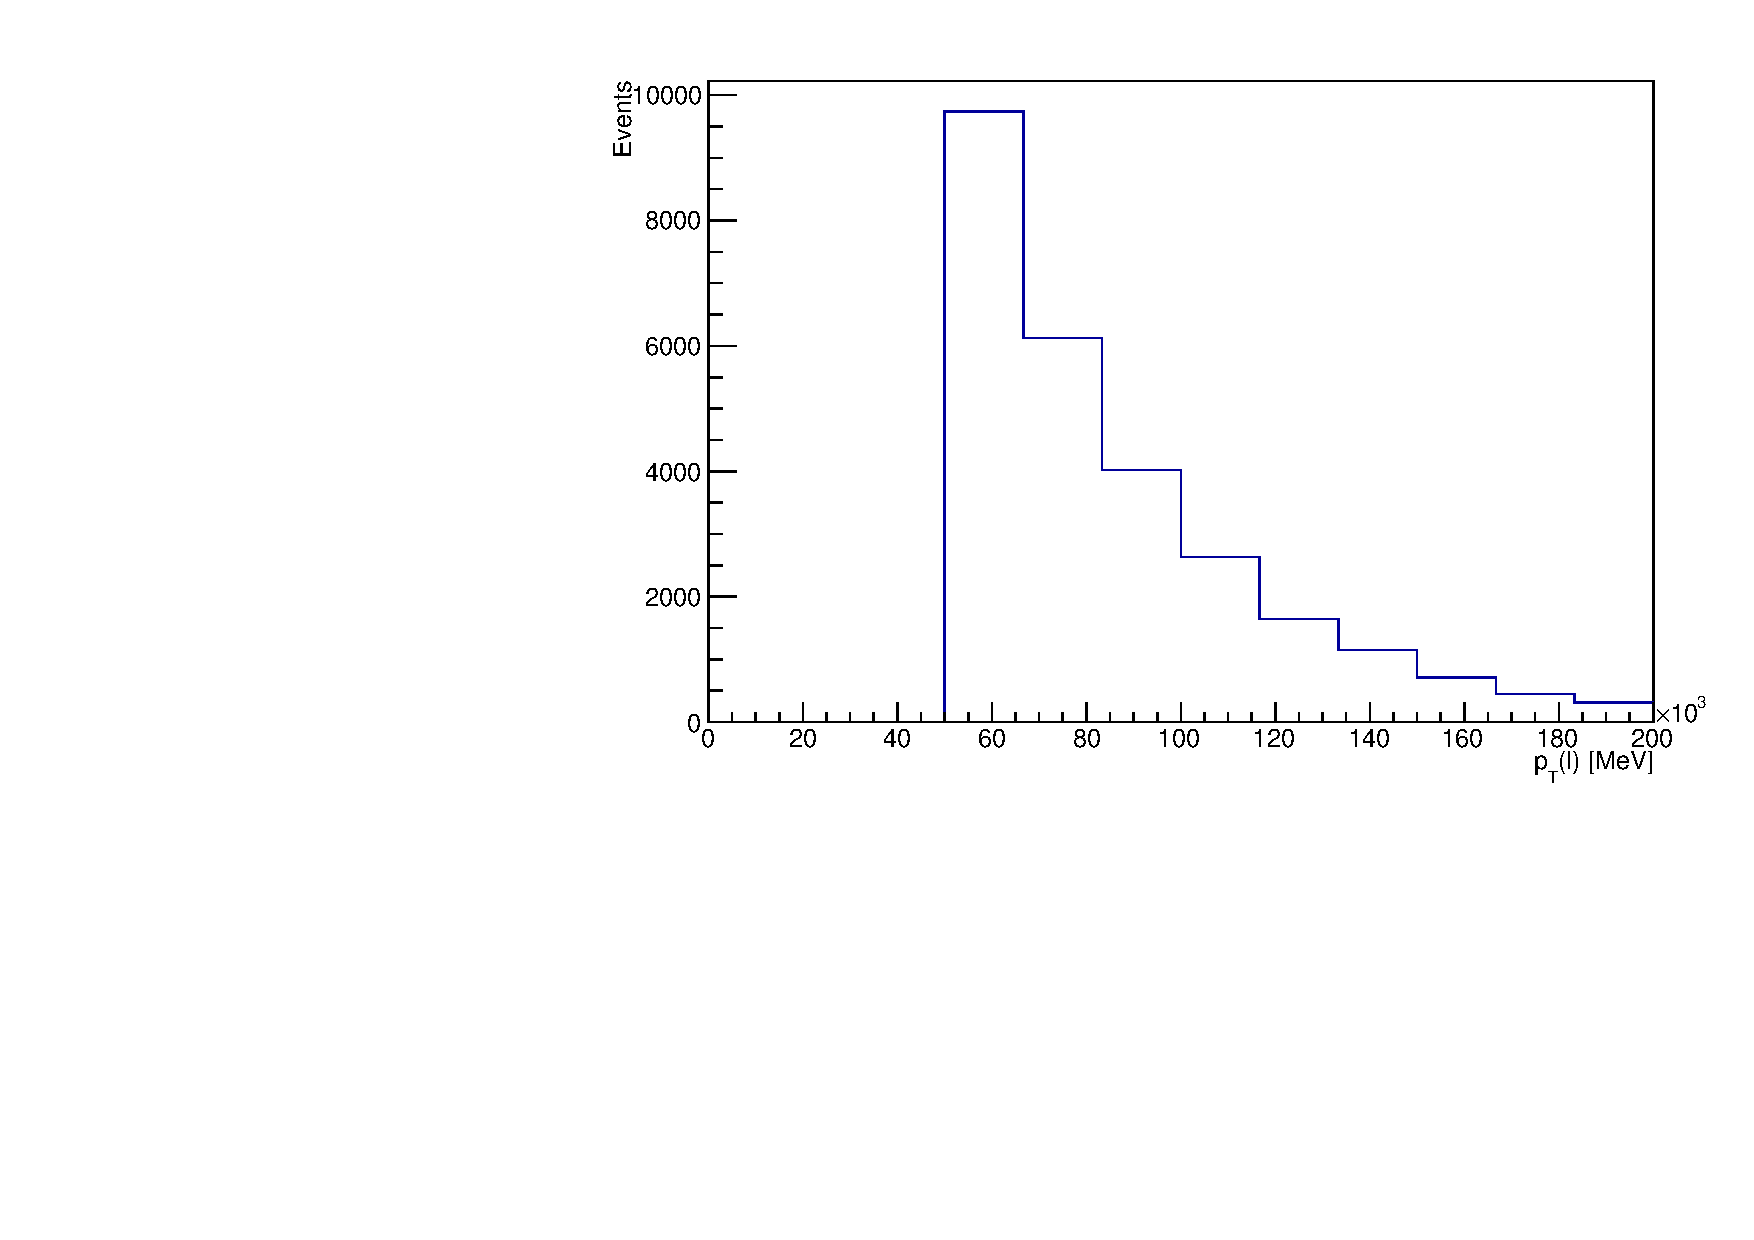
\includegraphics[width=\linewidth]{plots_and_txt/ttbar.mu_selected_/ttbar.mu_selected_lep_pt.pdf}
    \caption{}
    \label{fig:lep_pt}
  \end{subfigure}%
  \begin{subfigure}{0.5\textwidth}
    \centering
    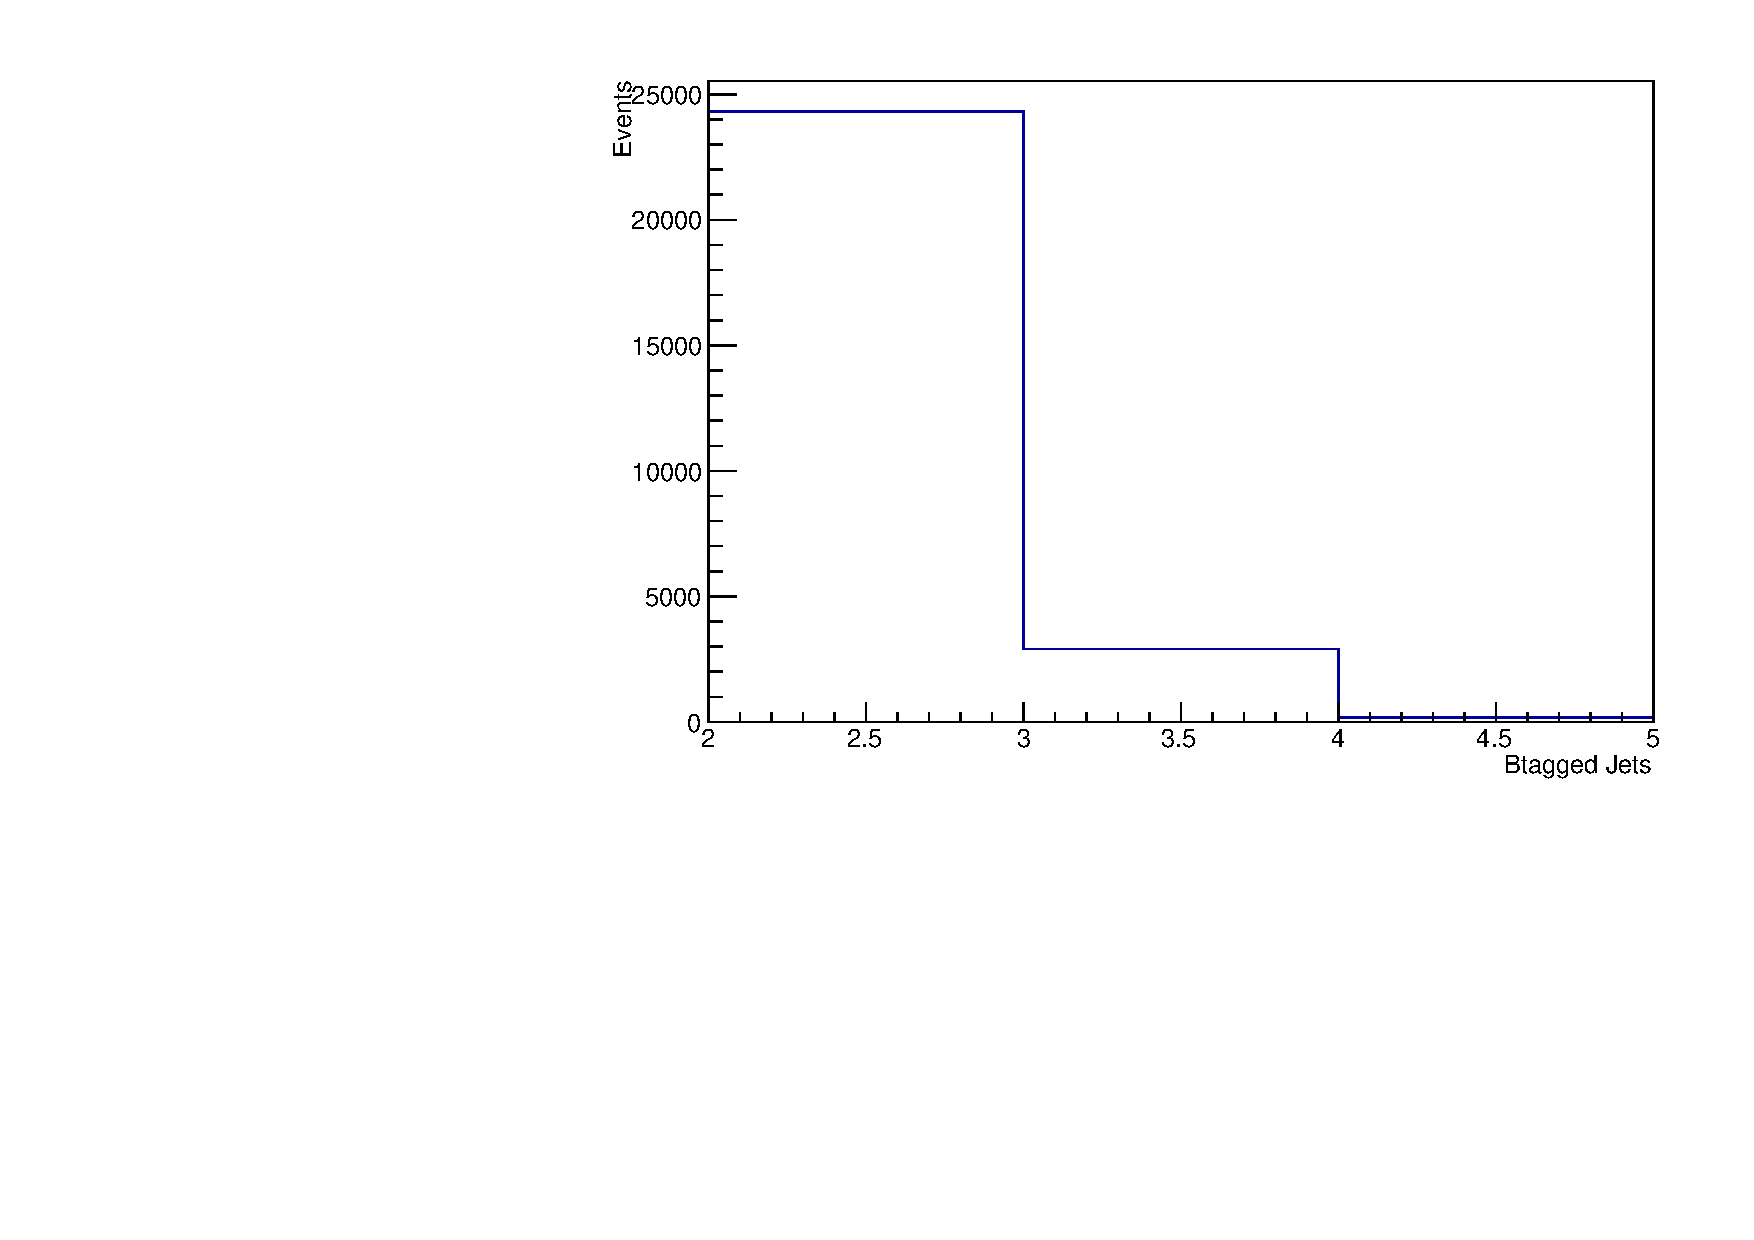
\includegraphics[width=\linewidth]{plots_and_txt/ttbar.mu_selected_/ttbar.mu_selected_btagged.pdf}
    \caption{}
    \label{fig:btagged}
  \end{subfigure}%
  \newline
  \begin{subfigure}{0.5\textwidth}
    \centering
    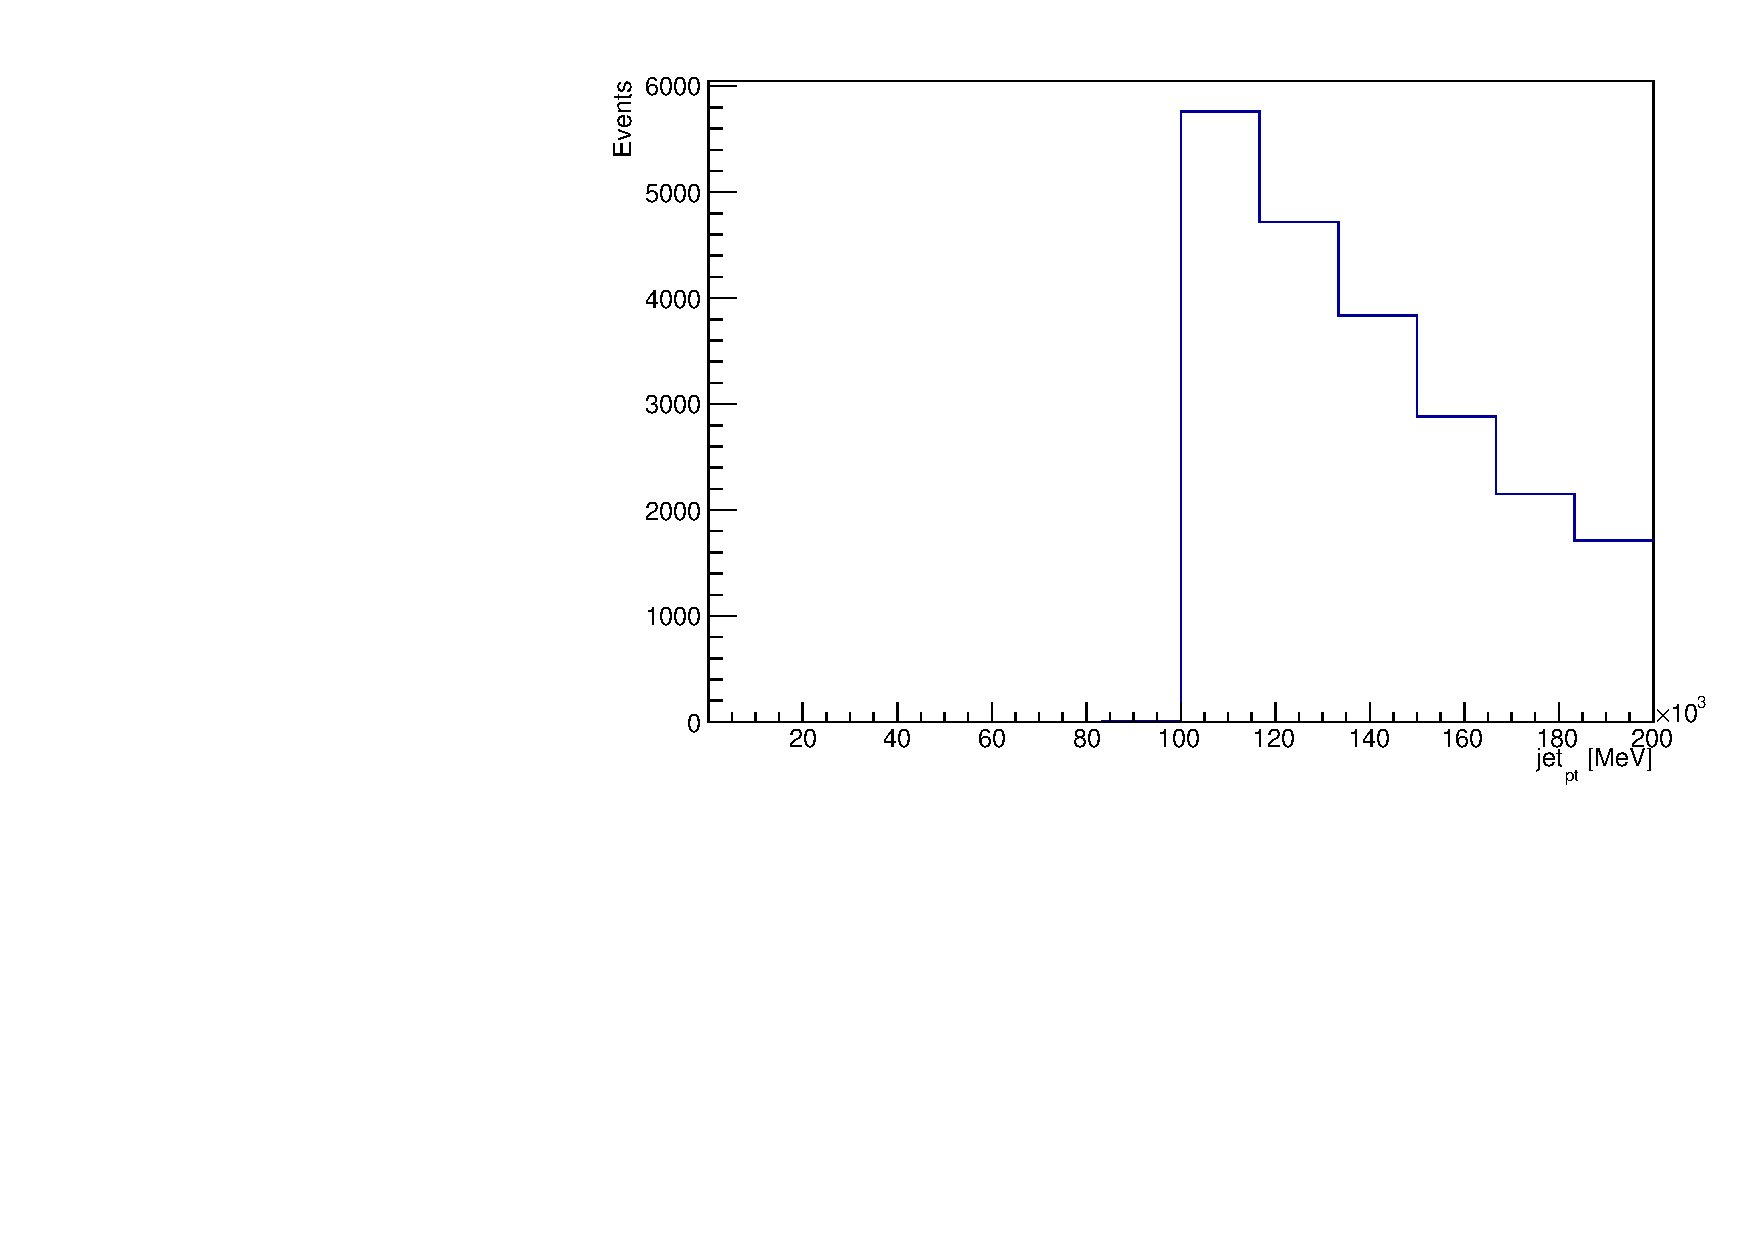
\includegraphics[width=\linewidth]{plots_and_txt/ttbar.mu_selected_/ttbar.mu_selected_jet_pt.pdf}
    \caption{}
    \label{fig:jet_pt_good}
  \end{subfigure}%
  \begin{subfigure}{0.5\textwidth}
    \centering
    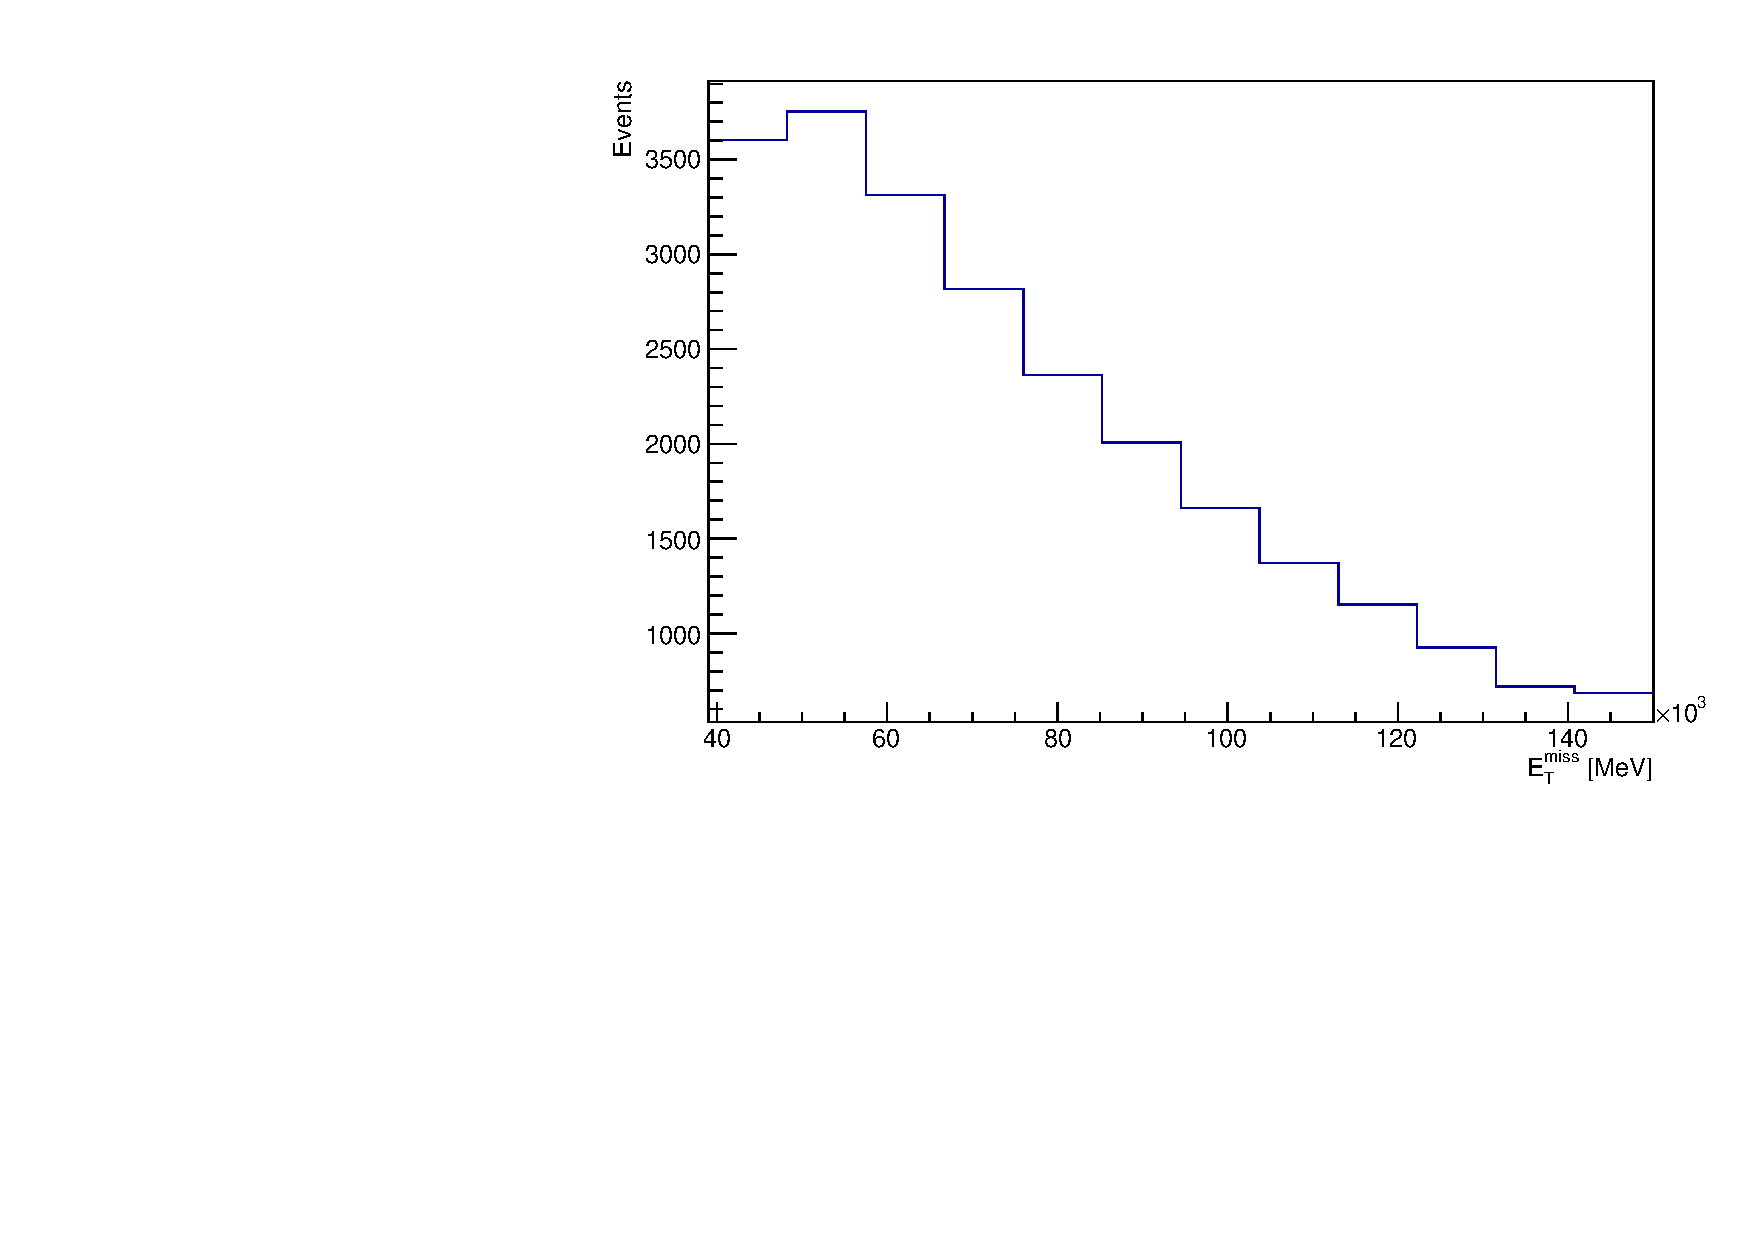
\includegraphics[width=\linewidth]{plots_and_txt/ttbar.mu_selected_/ttbar.mu_selected_met_et.pdf}
    \caption{}
    \label{fig:met_et}
  \end{subfigure}%
  \caption{Darstellung verschiedener Verteilungen der Größen der $t\bar{t}$ Monte-Carlo Simulation.
  Zu sehen sind der transverale Impuls der Myonen (\subref{fig:lep_pt}), die Anzahl an btagged Jets (\subref{fig:btagged}), der transverase Impuls des Jets mit dem höchsten transversalen Impuls des Events (\subref{fig:jet_pt_good}) und die fehlende transversale Energie (\subref{fig:met_et}).
  }
  \label{fig:Distributions}
\end{figure}

Auch nach der oben durchgeführten Selektion bleiben Untergrundprozesse wie der hier untersuchte $t\bar{t}$-Prozess übrig.
Um nun eine bessere Unterscheidung zwischen Signalereignissen, also $Z^\prime$-Ereignissen, und den Untergründen herzustellen werden weitere Größen konstruiert.
Da diese unter Umständen mehr Informationen als einfache Größen enthalten, kann ihre Diskriminierungsstärke deutlich erhöht sein.
Untersucht wurden $\Delta\Phi$, die Differenz zwischen dem Azimuthalwinkel der fehlenden Transversalenergie und der Leptonflugrichtung, die invariante Masse des Systems, die durch die drei Jets mit dem größten $p_T$ gebildet wird, die invariante Masse und die Pseudorapidität des Systems, die durch die vier Jets mit dem größten $p_T$, dem Lepton und dem Neutrino gebildet werden.
Für $\Delta\Phi$ wird darauf geachtet, dass jeweils die kleinere Differenz von $|\phi_1 - \phi_2|$ und $|2\pi - |\phi_1 - \phi_2||$ genutzt wird.
Diese werden für alle Datentupel und Monte-Carlo Simulationen berechnet.
Um die Größe mit der stärksten Diskriminierungsstärke zu ermitteln, werden die Verteilungen für den größten Untergrundprozess ($t\bar{t}$) mit einer möglichen Signalverteilung ($Z^\prime(1000)$, also einem hypothetischen $Z^\prime$ mit einer Masse von $\SI{1000}{\giga\electronvolt}$) verglichen.
Dies ist für die nachher gewählte Diskriminante, der vollständigen invarianten Masse des Systems, hier dargestellt.
Die restlichen Vergleiche sind im Anhang in Kapitel \ref{sec:reste} in Abbildung \ref{fig:Comparison1} - \ref{fig:Comparison3} zu sehen.

\begin{figure}
  \begin{subfigure}{0.5\textwidth}
    \centering
    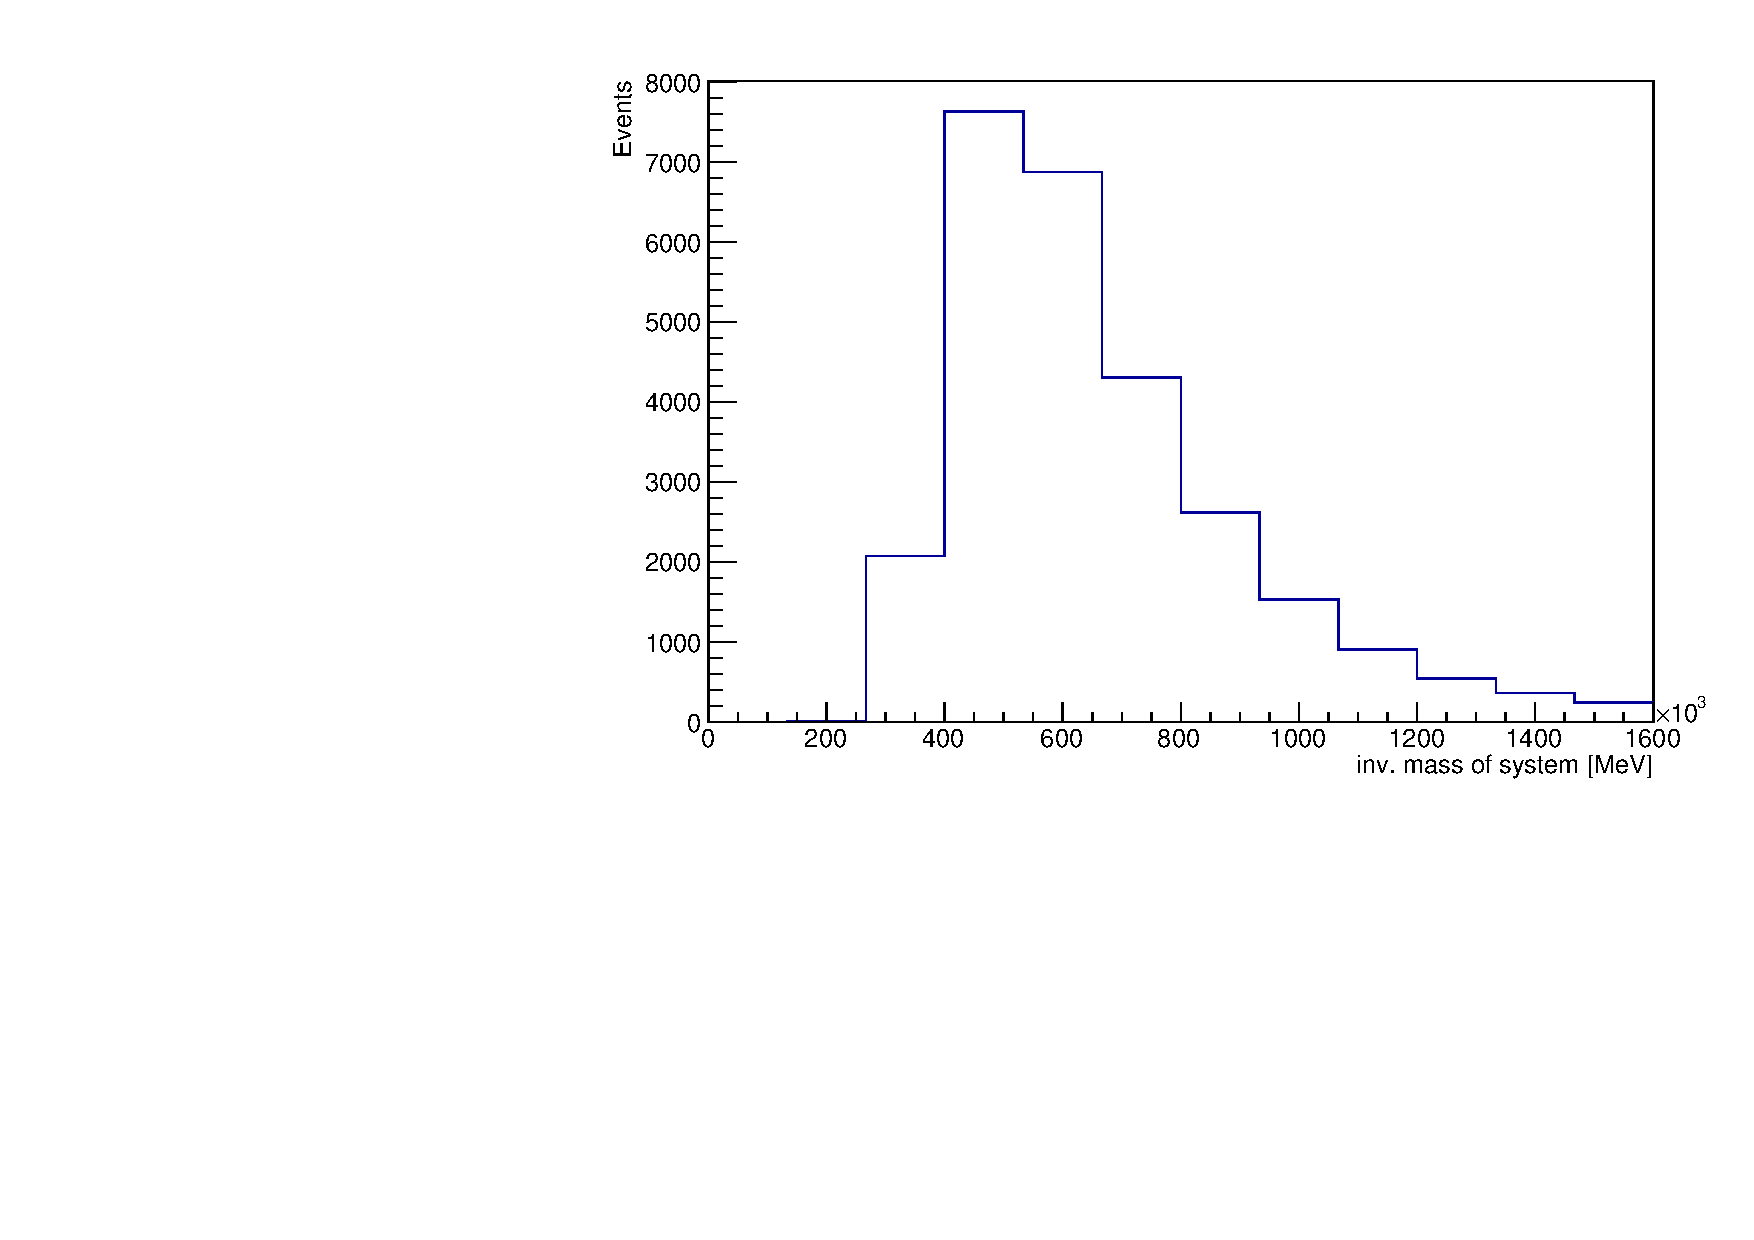
\includegraphics[width=\linewidth]{plots_and_txt/ttbar.mu_selected_/ttbar.mu_selected_SysJetMass.pdf}
    \caption{}
    \label{fig:ttbar_sys}
  \end{subfigure}%
  \begin{subfigure}{0.5\textwidth}
    \centering
    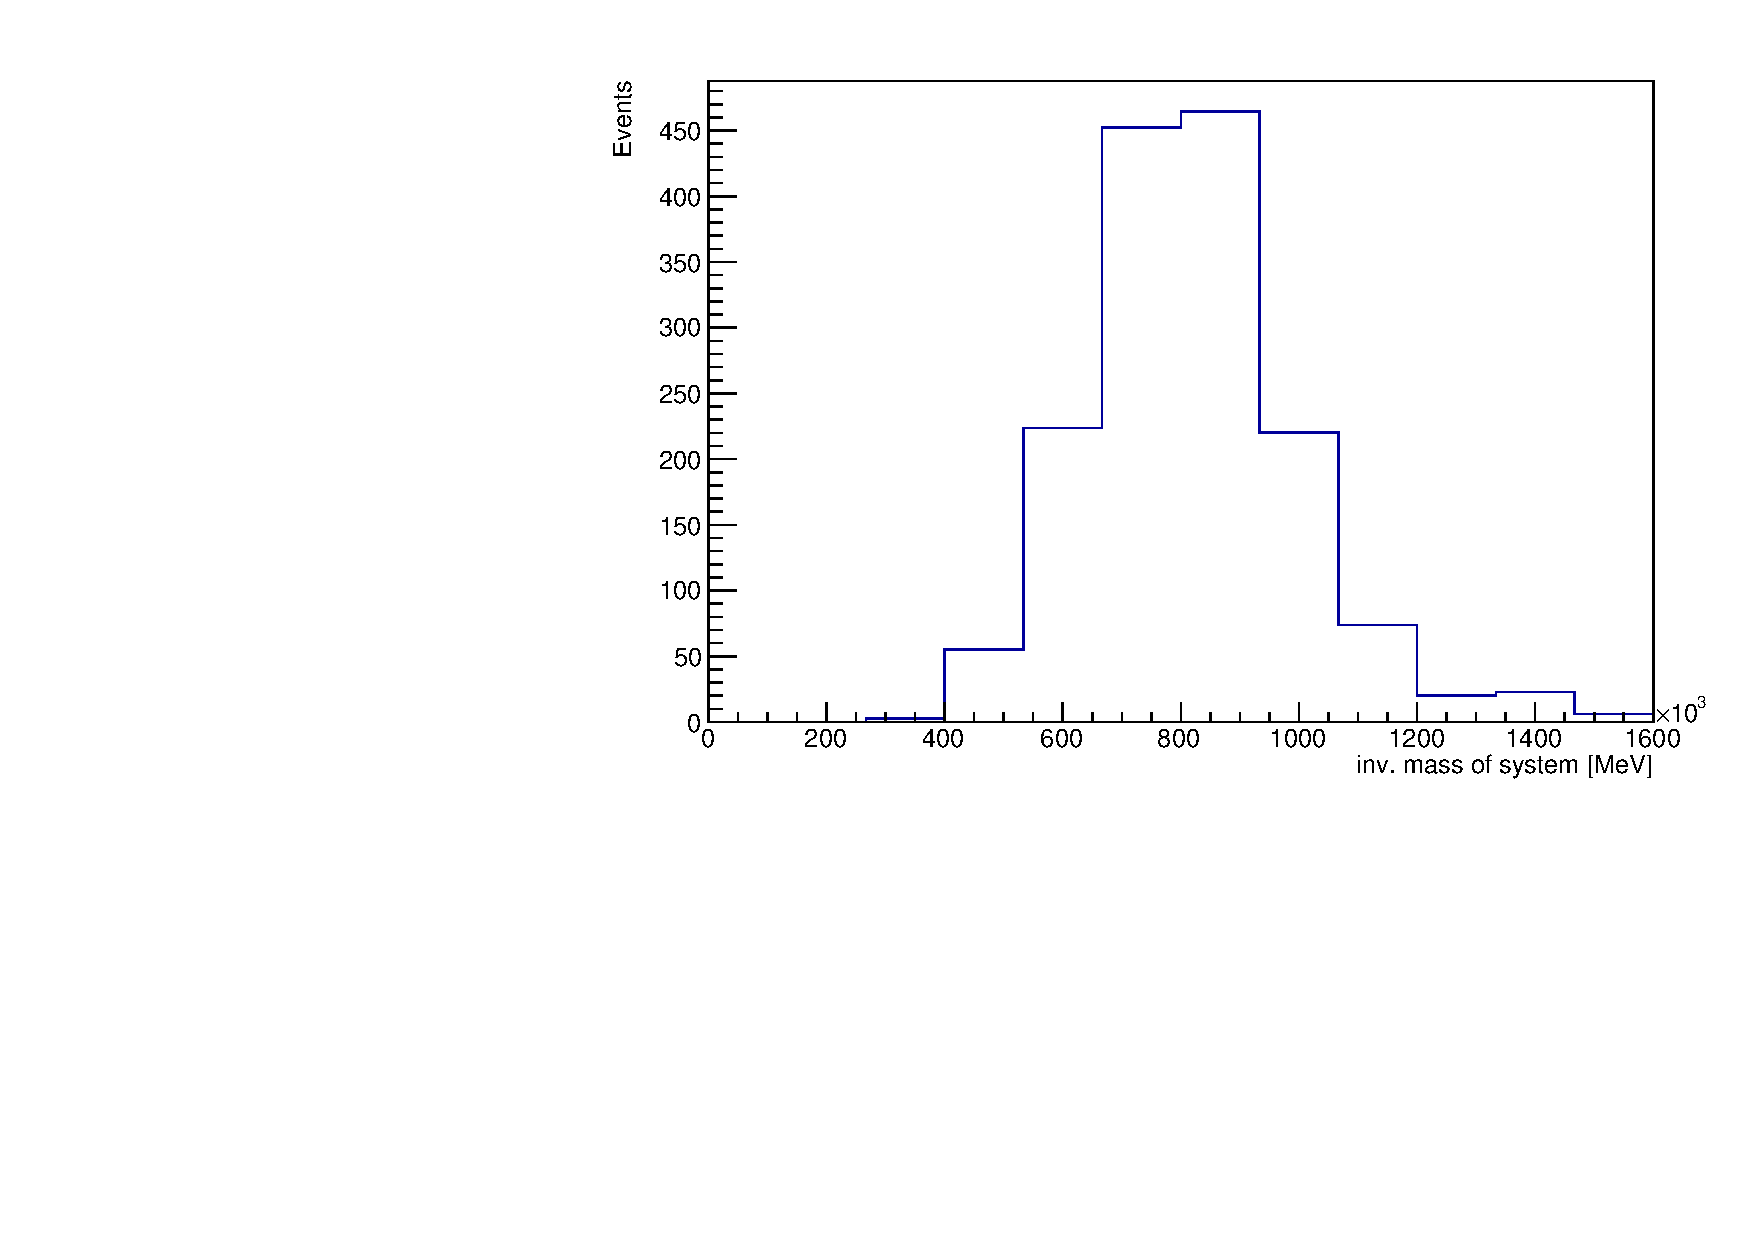
\includegraphics[width=\linewidth]{plots_and_txt/zprime1000.mu_selected_/zprime1000.mu_selected_SysJetMass.pdf}
    \caption{}
    \label{fig:zprime_sys}
  \end{subfigure}%
  \caption{Vergleich der Verteilung der invarianten Masse des Systems, welches aus den vier Jets mit dem größten $p_T$, dem Lepton und dem Neutrino gebildet wird.
  Dies ist für die $t\bar{t}$-Untergrundsimulation \subref{fig:ttbar_sys} und der Signalsimulation des $Z^\prime(1000)$ \subref{fig:zprime_sys} dargestellt.
  Diese Größe dient weiter als Diskriminante.
  }
  \label{fig:Comparison}
\end{figure}













%-

